\subsection{Road Generator}
\begin{center}
  \textit{Terrain, Population map} $\rightarrow$ \textbf{RoadGenerator} $\rightarrow$ \textit{Road network} 
\end{center}
Road generation is what will design the entire frame of the city, and it will do it by placing different kinds of roads.
The size of each city will be defined by the user through the population markers.
Cities far away from each other will be connected by highways, and along those highways, there is a chance that small villages are generated.
The roads will be constructed using Agent-based generation.



\subsubsection{Plotting Cities}
The user should be able to specify exactly where cities should begin their generation sequence.
They will do this via population markers.
Each city has a type that describes the general appearance and layout of the city.
Some examples of city type generation strategies are;
\begin{itemize}
  \item Paris strategy, which would generate circular cities with roads extending from the middle and outwards.
  \item Manhattan strategy, which consists of lots of straight roads going through the city perpendicular to other roads, creating a grid-like appearance.
  \item Chaotic strategy, completely random with lots of turning, no structure whatsoever.
\end{itemize}

Multiple cities can be plotted out at once, and generally, when a road leaves the bounds of the city it converts to a highway that aims to connect to other denser areas.

\begin{center}
  \begin{figure}[H]
    \centering
    \begin{subfigure}[b]{0.49\textwidth}
      \frame{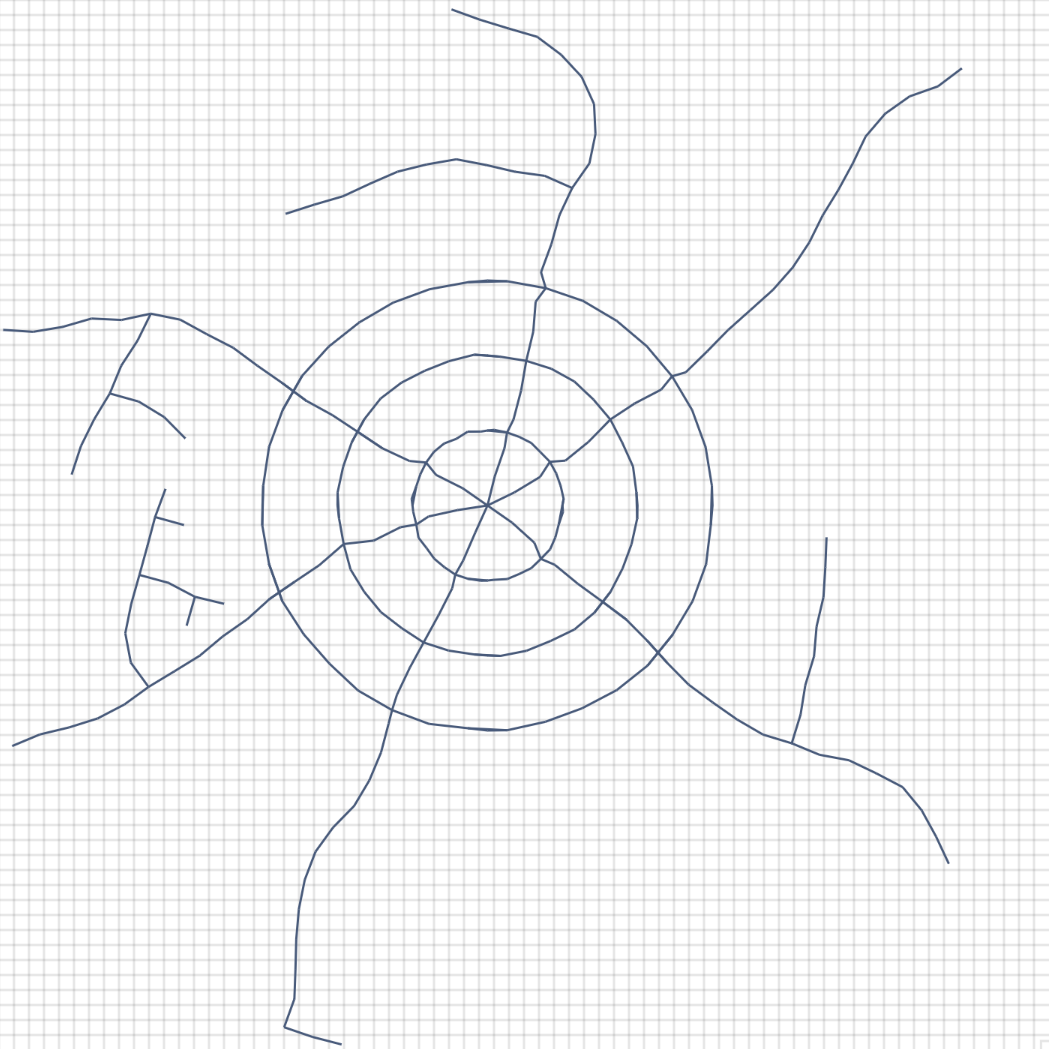
\includegraphics[width=\linewidth]{figure/gen_road_paris_main.png}}
      \caption{Main road generation}
      \label{fig:gen_road_paris_main}
    \end{subfigure}
    \begin{subfigure}[b]{0.49\textwidth}
      \frame{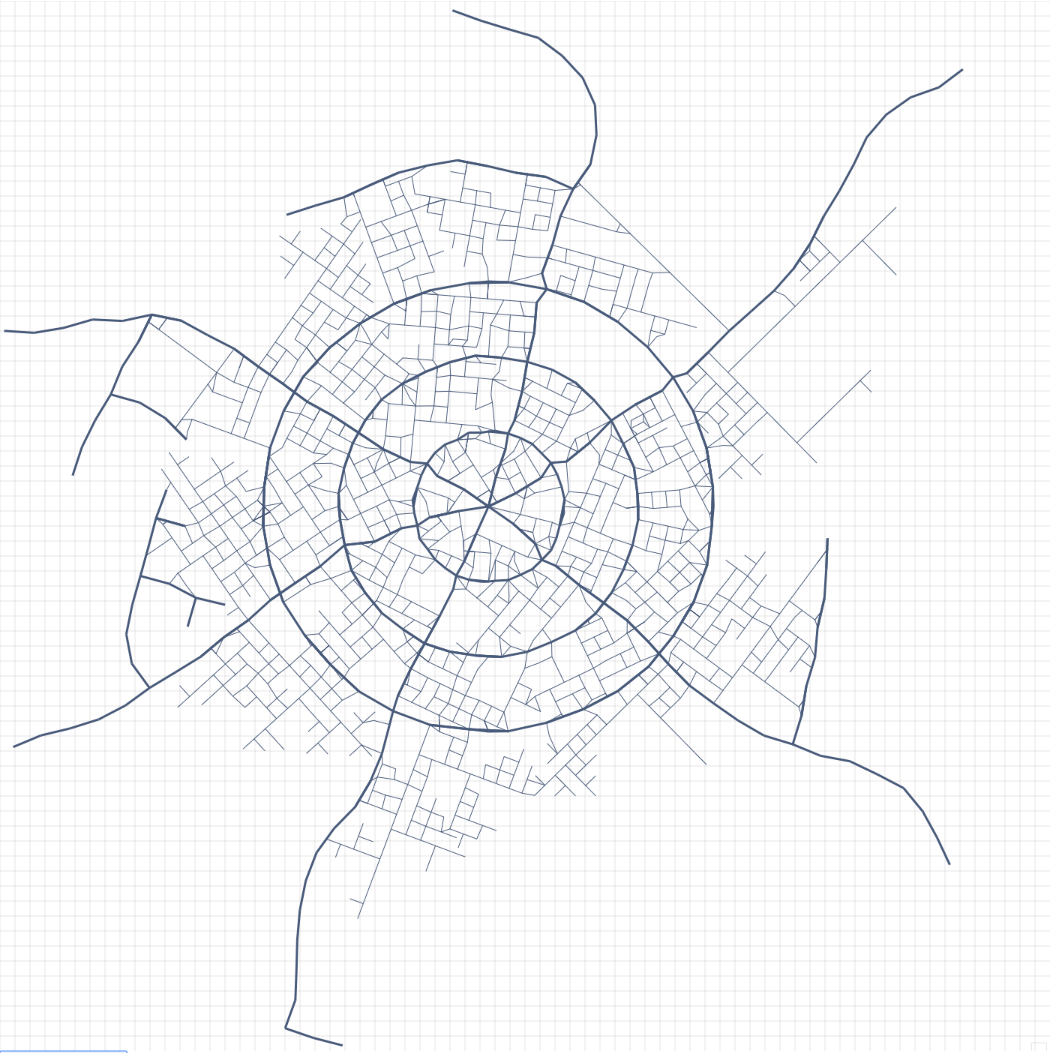
\includegraphics[width=\linewidth]{figure/gen_road_paris_streets.png}}
      \caption{Streets generation}
      \label{fig:gen_road_paris_streets}
    \end{subfigure}
    \caption{Visualization of the Paris road generation strategy}
    \label{fig:gen_road_paris_visualization}
  \end{figure}
\end{center}

\subsubsection{Main Road Generation}
Main roads, and roads in general, are generated by what is called \textit{Agents}.
These only have two jobs.
The first is to walk around the terrain and leave roads behind them.
The second is to spawn new agents to branch for the existing agent.
The agents generate the main roads depending on if it is inside a city, and what type of city it is.
All agents have a strategy that they will follow, instructing them how they should move around.
Agent strategies also tell the agent when it should terminate.

This type of generation results in a lot of flexibility, because each agent can be instructed to walk around differently.
For the Paris strategy, some agents are configured to walk around in circles around the center point and others are configured to walk roughly straight outwards from the center.
For the Manhattan strategy, the agents simply create completely straight roads, some agents are rotated by 90 degrees to create the perpendicular roads.

This also means agents can decide to switch strategy depending on some criteria, for example when an agent leaves the bounds of a city, it can change its strategy to a highway-type strategy.

Highways are a type of the main road, and agents that have a strategy that creates highways should attempt to follow the population map towards higher density areas.
This will be done through gradient ascent on the population map.
This helps cities to connect because highways generally do not turn around as much as other main roads and it will eventually find a higher density area in the population map to go towards.

However, higher-density areas do not mean there is always a city located there, it might find an area without a city.
The idea is that the highway strategy can also create new cities or villages if it comes across a very dense area and has not connected to an existing city.
There are cases where a city can be created right next to another city, but that would just result in both cities merging into one.

While generating main roads, new agents are created which branch off the main road to create streets.

\subsubsection{Street Generation}
While generating main roads, new agents are created that branch off the main road to create streets.
These are generally straight and grid-like, to mimic the patterns found in most neighborhoods.
However, different kinds of street strategies can be created to mimic other types of neighborhoods as well.
To ensure that streets do not cut off main roads, these agents are given a lower priority which ensures that they are always created after main roads are finished generating.
The agents are then prioritized according to the order they were created, which means an agent will generate an entire neighborhood before the next street agent begins.
This creates clearer patterns around the city with fewer agents competing over the same area.

Agents with a street strategy will always look up the population map before placing a road or branching.
Higher density means a higher chance of branching, creating denser neighborhoods near the center of the city.
An agent that tries to travel into a place with too little of a population density will simply terminate without creating a road. 
